\documentclass[12pt, a4paper] {ncc}
\usepackage[utf8] {inputenc}
\usepackage[T2A]{fontenc}
\usepackage[english, russian] {babel}
\usepackage[usenames,dvipsnames]{xcolor}
\usepackage{listings,a4wide,longtable,amsmath,amsfonts,graphicx,tikz}
\usepackage{pgfplots}
\usepackage{indentfirst}
\usepackage{bytefield}
\usepackage{multirow}
\usepackage{tabularx}

\usepackage[left=1.5cm,right=1.5cm,top=2cm,bottom=1.5cm,bindingoffset=0cm]{geometry}

\begin{document}
\setcounter{figure}{0}
\frenchspacing
\pagestyle{empty}
\begin{center}
     Национальный исследовательский университет информационных технологий,
                              механики и оптики\\
                        Кафедра вычислительной техники\\
                          Сети ЭВМ и телекоммуникации
\end{center}
\vspace{\stretch{2}}
\begin{center}
                            Учебно-исследовательская работа №5\\
                <<Технологии QoS в компьютерных сетях>>
\end{center}
\vspace{\stretch{3}}
\begin{flushright}
                                          Студентка:\\
										  Преподаватель:\\
														 {\it Шинкарук Д.Н. }
\end{flushright}
\vspace{\stretch{4}}
\begin{center}
                             Санкт-Петербург, 2017
\end{center}
\newpage

\section*{Цели работы}
    Цель работы -- изучение эффективности приоритезации трафика для управления качеством обслуживания
	(Quality of Service, QoS) в компьютерных сетях.     

\section*{Исходные данные}

	\begin{itemize}
		\item Пропускная способность: N = 5 Mbps.
        \item Размер буфера: S = 7 Kb.
		\item Приоритеты WFQ: $W_1:W_2 = 7:1$, $W_1 = 0.86$ $W_2 = 0.14$
	\end{itemize}

	\begin{table}[h!]
		\begin{tabular}{|c|c|c|}
			\hline
			Параметры	       & Skype & Twitch  \\ \hline
			Задержка, ms       & 100   &  1000   \\ \hline
			Джиттер, ms        & 50    &  -  	 \\	\hline
			Потеря пакетов, \% & 0.1   & 0.1     \\ \hline
		\end{tabular}
	\end{table}

	
\section*{Захват трафика}

	Захват VoIP трафика происходил следующим образом: определение открытых программой Skype портов,
	определение, через какой порт и на какой адрес происходит наибольшая активность при звонке,
	захват трафика c фильтром \texttt{port PORT and host HOST and udp}.

	\begin{figure}[h!]
    	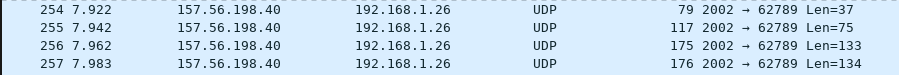
\includegraphics[scale=0.5]{./img/skype_pcap.png}
	\end{figure}

	Захват VoD трафика происходил следующим образом: определение адреса, через который идёт
	видео-трафик, с помощью отладочной консоли браузера; захват трафика c фильтром 
	\texttt{host HOST and tcp}.
	\begin{figure}[h!]
    	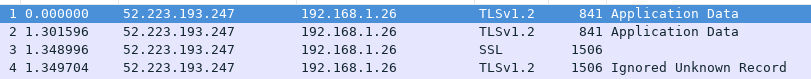
\includegraphics[scale=0.5]{./img/twirch_pcap.png}
	\end{figure}

\newpage
\section*{Функции распределения интервалов между пакетами}

	\begin{figure}[h!]
    	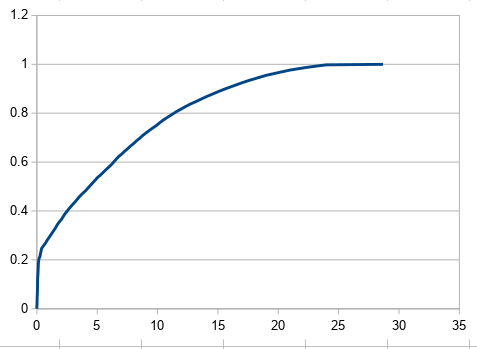
\includegraphics[scale=0.4]{./img/skype_inter_distr.png}
		\caption{Skype}
	\end{figure}
	\begin{figure}[h!]
    	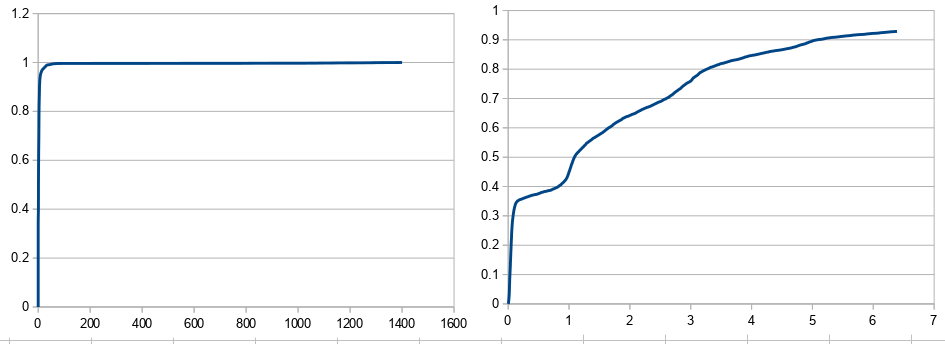
\includegraphics[scale=0.4]{./img/twitch_inter_dist.png}
		\caption{Twitch}
	\end{figure}

\section*{Функции распределения размеров пактов}

	\begin{figure}[h!]
    	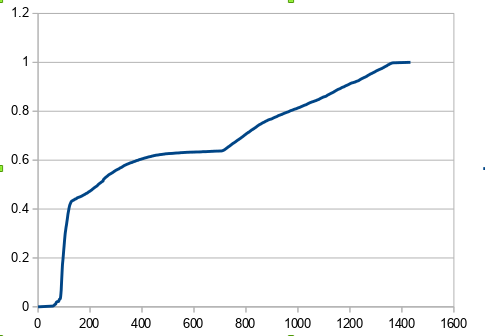
\includegraphics[scale=0.5]{./img/skype_size_distr.png}
    	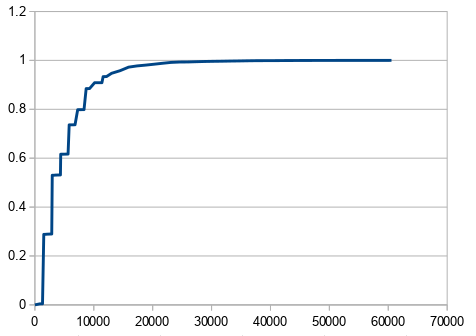
\includegraphics[scale=0.5]{./img/twitch_size_dist.png}
		\caption{Skype и Twitch}
	\end{figure}

\section*{Эксперименты}
	\subsection*{Исследование FIFO}
        Элементарная очередь без приоретизации: каждый класс трафика получает одинаковое количество
        обслуживания в случае, если считать задержку ожидания в буфере; при учёте задержки при выдаче
        в канал связи, то равное обслуживание не обеспечивается. 

		\begin{figure}[h!]
			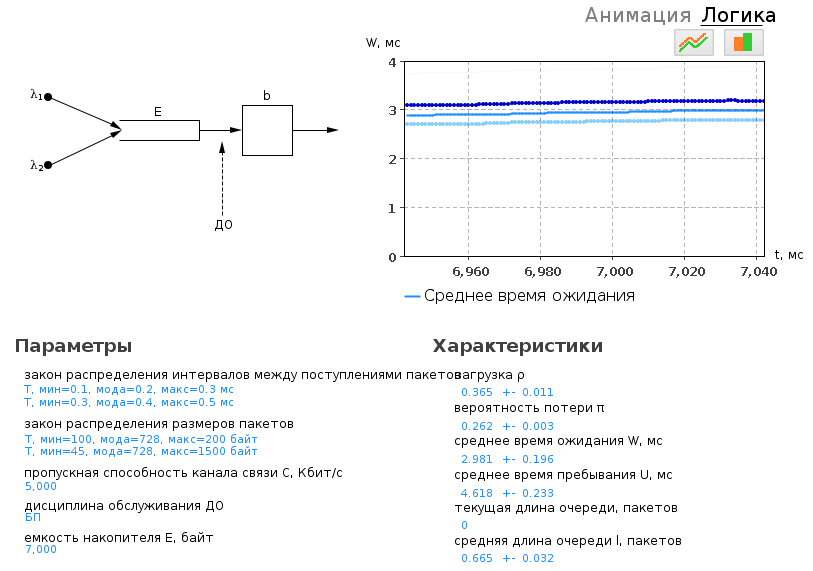
\includegraphics[scale=0.5]{./img/fifo_5000_7000.png}
		\end{figure}
		При вариации значения пропускной способности не удалось добиться характеристик, соответствующих
		заданным требованиям. Такое поведение обуславливается большим размером пакетов и малым интервалом
		между времени между пакетами: заданного в задании размера буфера и пропускной способности недостаточно
		для данного типа трафика. При попытке увеличить исходные параментры были получены следующие результаты.
		\begin{figure}[h!]
			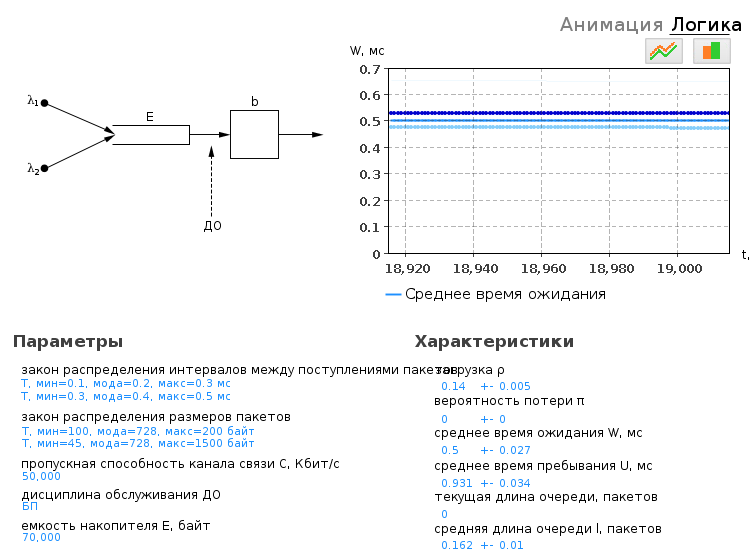
\includegraphics[scale=0.5]{./img/fifo_50000_70000.png}
		\end{figure}
		\begin{figure}[h!]
			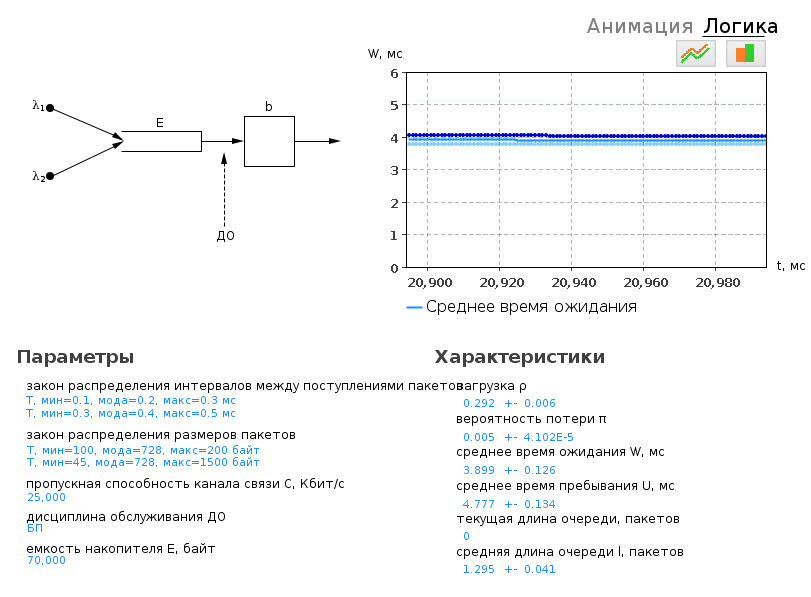
\includegraphics[scale=0.5]{./img/fifo_25000_70000.png}
		\end{figure}
		\newpage
		Графики изменений значений загрузки, вероятности потерь и времени ожидания в зависимости от
        пропускной способности.
		\begin{figure}[h!]
			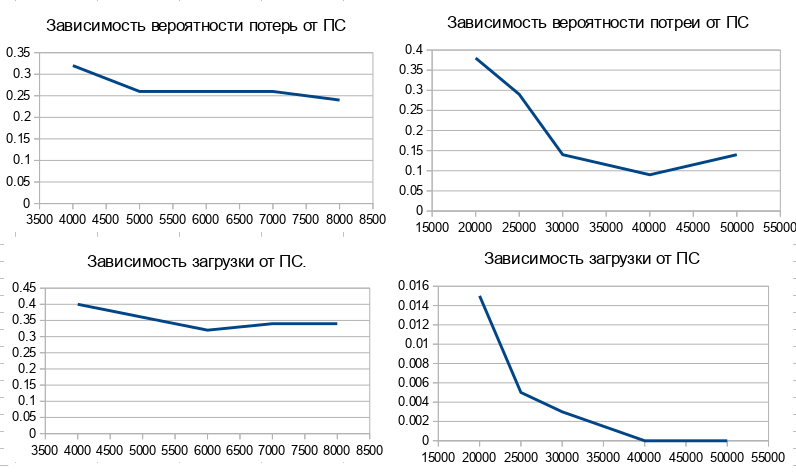
\includegraphics[scale=0.5]{./img/fifo_cmp1.png}
			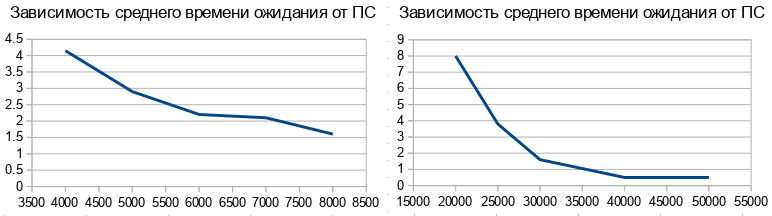
\includegraphics[scale=0.5]{./img/fifo_cmp2.png}
			\caption{Слева показатели при объёме 7Kb, справа -- 70 Kb.}
		\end{figure}
		
		\newpage
		Из графиков видно, что при объеме буфера в 7Kb при вариации ПС показатели практически не изменились, в то
		время как при объёме в 70Kb удалось найти пропускную способность (25000 bps), при которой характеристики
		соответствуют требуемым.

%	\newpage
	\subsection*{Исследование PQ}
        Разным классам трафика устанавливается приоритет: трафик низкоприоритетного класса передаётся только в том случае,
        когда нет пакетов высокоприоритетного класса на передачу. Таким образом обуславливается наилучшее качество обслуживания
        для высокоприоритетного класса, однако блокирует низкоприоритетный при перегрузках.

		\begin{figure}[h!]
			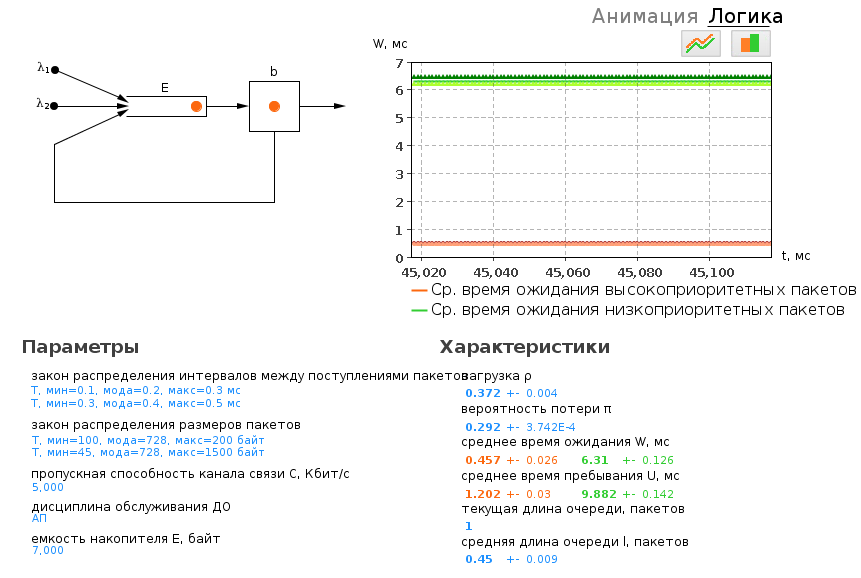
\includegraphics[scale=0.5]{./img/pq_5000_7000.png}
		\end{figure}
		\newpage
		Как и прошлом случае, при вариациии ПС добиться требуемых качеств не удаётся. 

		\begin{figure}[h!]
			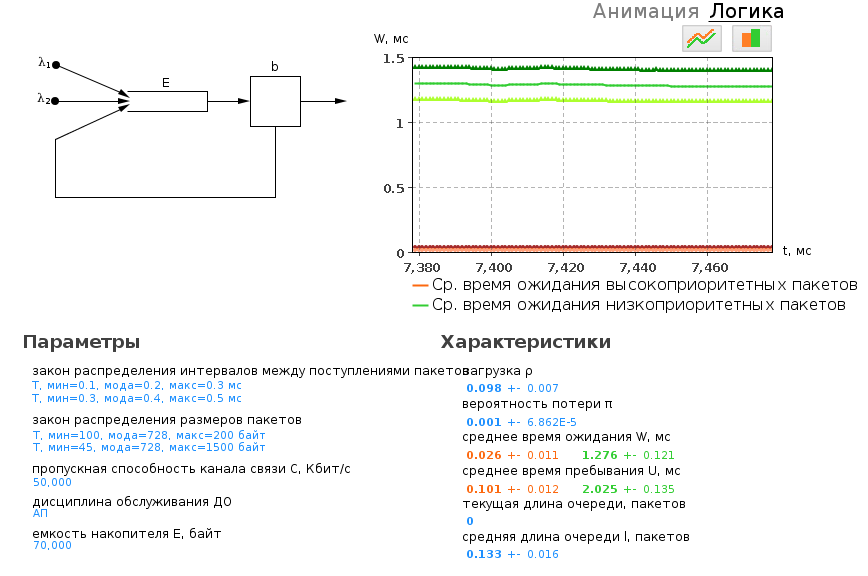
\includegraphics[scale=0.5]{./img/pq_50000_70000.png}
		\end{figure}
		\begin{figure}[h!]
			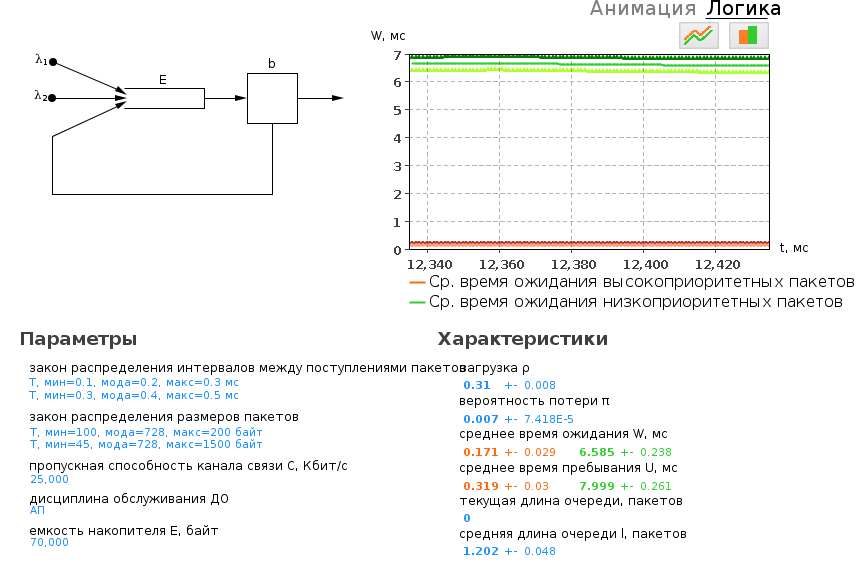
\includegraphics[scale=0.5]{./img/pq_25000_70000.png}
		\end{figure}

		\newpage
		Графики изменений значений загрузки, вероятности потерь и времени ожидания в зависимости от
        пропускной способности.
		%\newpage
		\begin{figure}[h!]
			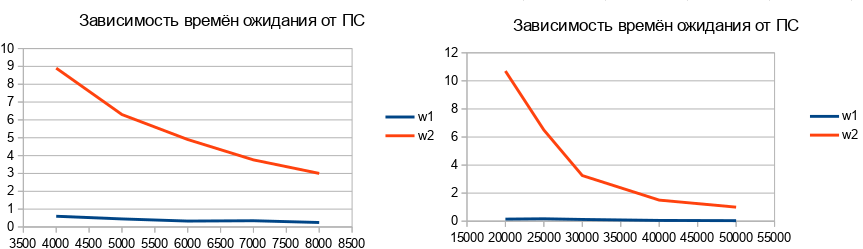
\includegraphics[scale=0.4]{./img/pq_cmp1.png}
		\end{figure}
		\begin{figure}[h!]
			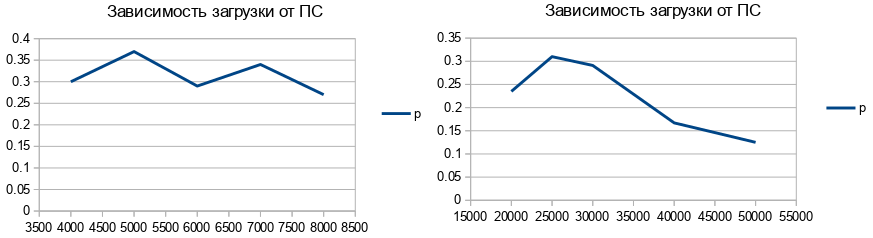
\includegraphics[scale=0.4]{./img/pq_cmp2.png}
		\end{figure}
		\begin{figure}[h!]
			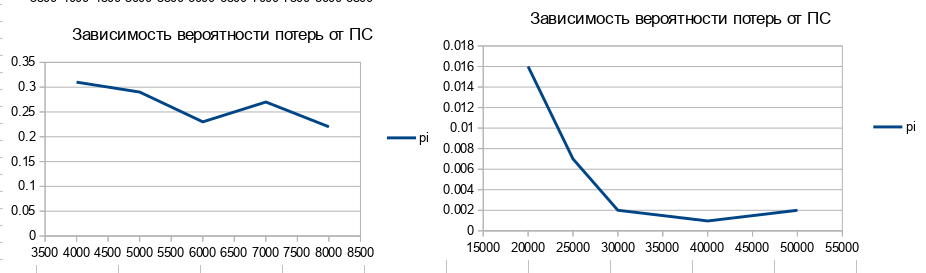
\includegraphics[scale=0.4]{./img/pq_cmp3.png}
			\caption{Слева показатели при объёме 7Kb, справа -- 70 Kb.}
		\end{figure}

		Из графиков видно, что изменение ПС сильно влияет на низкоприоритетный трафик. 


	\subsection*{Исследование WFQ}

        Для каждого трафика устанавливается вес; за каждый цикл работы WFQ из очереди одного класса передаются пакеты
        суммарным размером равным весу класса. Установка веса даёт гарантии, что класс с большим весом будет получать
        большее качество обслуживания и что в условиях высокой нагрузки класс будет получает канал за конечное время.

		\begin{figure}[h!]
			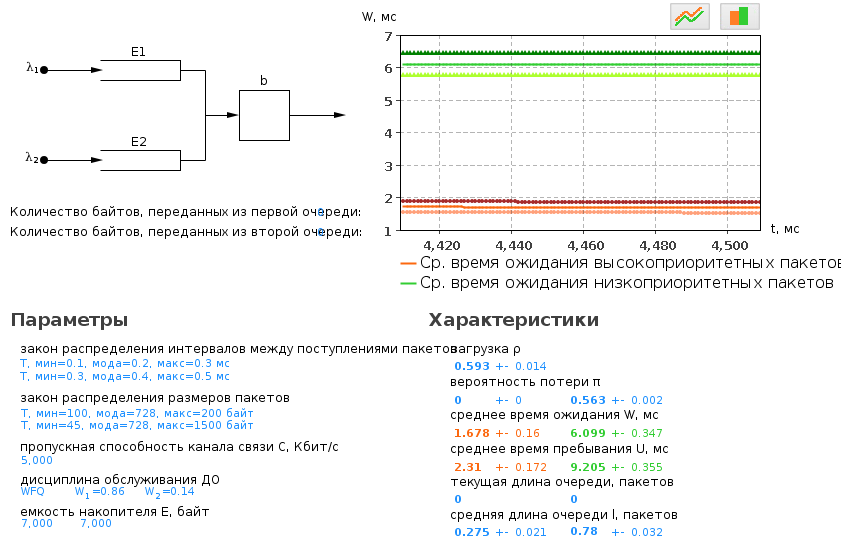
\includegraphics[scale=0.5]{./img/wfq_5000_7000.png}
		\end{figure}

		При варьировании весов результаты незначительно улучшились. 

		\begin{figure}[h!]
			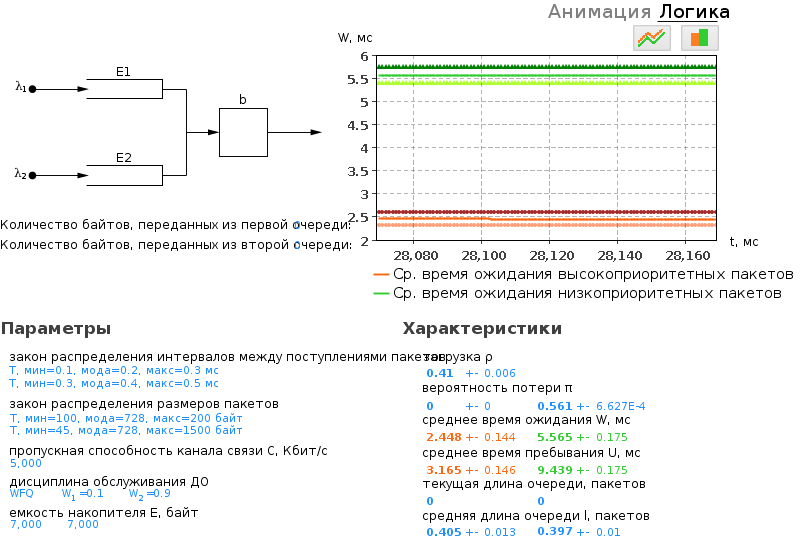
\includegraphics[scale=0.5]{./img/wfq_5000_7000_w19.png}
		\end{figure}

		Как и прошлом случае, при вариациии ПС добиться требуемых качеств не удаётся. 

		\begin{figure}[h!]
			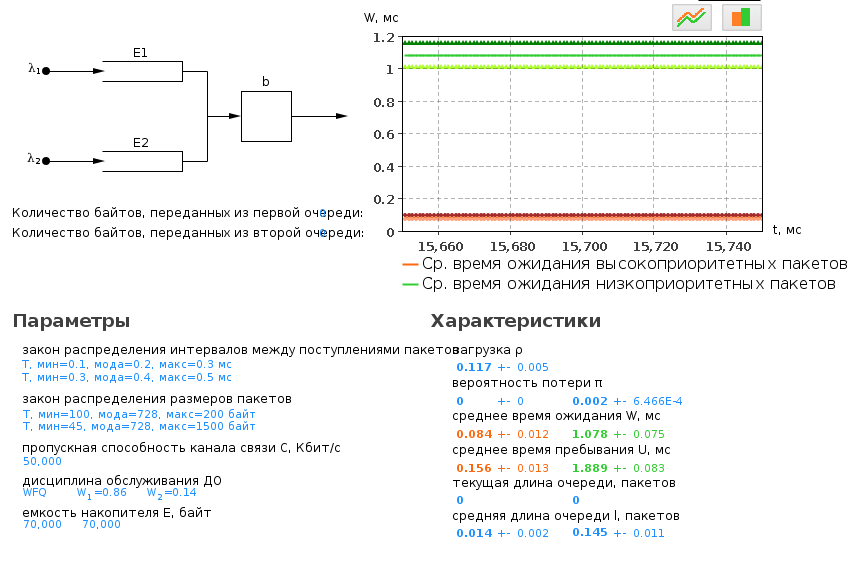
\includegraphics[scale=0.5]{./img/wfq_50000_70000.png}
		\end{figure}
		\begin{figure}[h!]
			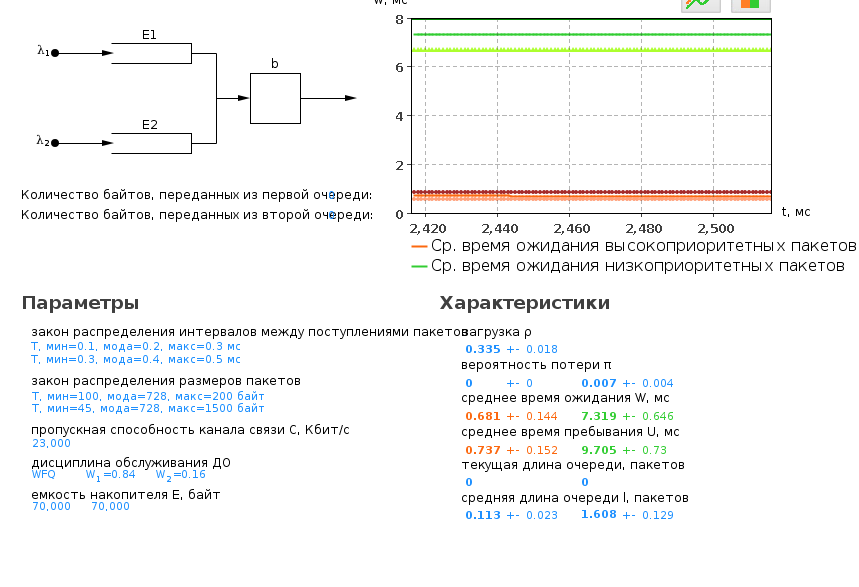
\includegraphics[scale=0.5]{./img/wfq_23000_70000.png}
		\end{figure}
		\newpage	
		Наименьшее значение ПС удалось достичь при 23000 bps. При варьировании весов на данной пропускной способности
		и на ряде значений ниже не удалось добиться значительно лучших результатов.

		\newpage
		Графики изменений значений загрузки, вероятности потерь и времени ожидания в зависимости от
        пропускной способности.
		\begin{figure}[h!]
			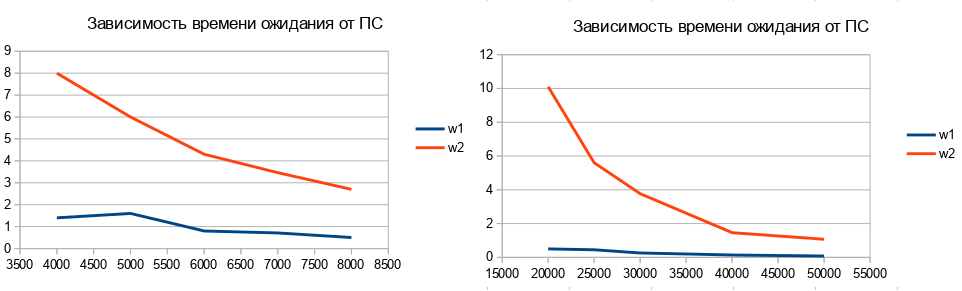
\includegraphics[scale=0.4]{./img/wfq_cmp1.png}
			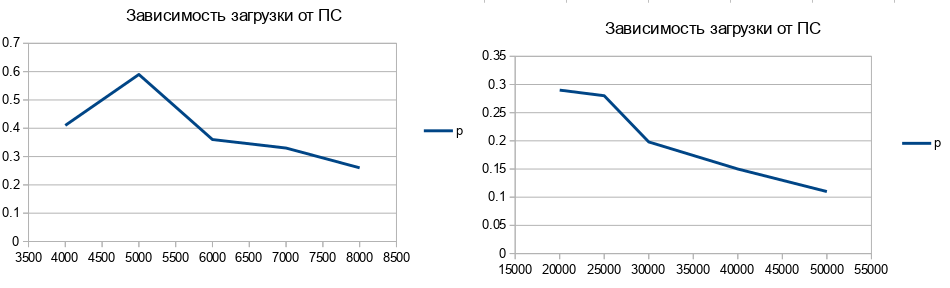
\includegraphics[scale=0.4]{./img/wfq_cmp2.png}
			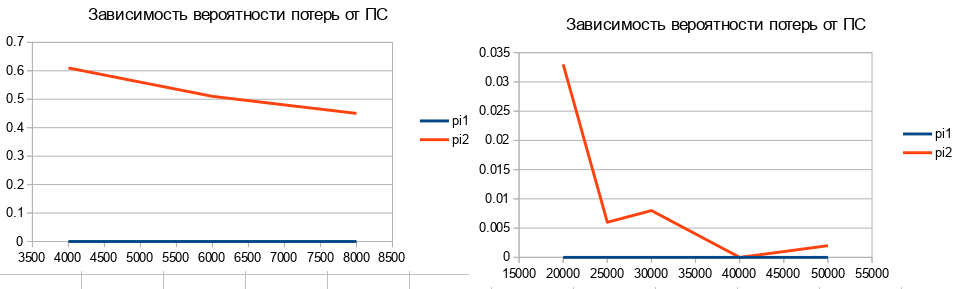
\includegraphics[scale=0.4]{./img/wfq_cmp3.png}
			\caption{Слева показатели при объёме 7Kb, справа -- 70 Kb.}
		\end{figure}

		В сравнении с PQ в режиме перегрузки (S=7Kb, N=2Mbps).
		\begin{table}[h!]
			\begin{tabular}{|c|c|c|c|c|c|c|c|}
				\hline
				ДО 		        &		$w_1$	& $u_1$  &  $w_2$   & $u_2$  & $p$   & $\pi_{1}$ &  $\pi_{2}$ \\ \hline
                PQ      		& 0.9           & 1.5    & 300      & 314    & 1     & 0.6       &  -   \\ \hline 
                WFQ(0.86,0.14)  & 33.2          & 34.1   & 148      & 151    & 1     & 0.4       & 0.89 \\ \hline
                WFQ(0.14,0.86)  & 198.9         & 201    & 30       & 32     & 1     & 0.89      & 0.75 \\ \hline
                WFQ(0.5,0.5)    & 51.6          & 52.4   & 57.1     & 58.3   & 1     & 0.6       & 0.8  \\ \hline 
			\end{tabular}
		\end{table}

\section*{Вывод}

В ходе проведения учебно-исследовательской работы было подмечено следующее:
\begin{enumerate}
	\item Выданная для проведения исследований модель содержала ошибку: при выборе ДО WFQ значения времени ожидания
		  и времени пребывания в очереди не обновлялись. Баг обусловлен тем, что при выходе из источников (source)
		  не устанавливалось свойство объекта (entity.priority), которое влияет на изменение обозначенных выше показателей.
	\item При захвате трафика VoD обнаружилось, что размер пойманных TCP-пакетов не соответствует размеру MTU. Скорее всего,
		  это происходит из-за механихма GSO (generic segmentation offload), при котором фрагментация и дефрагментация пакетов
		  происходит в обход CPU на сетевых интерфейсах. Однако настроить получение пакетов без этого мехнизма не получилось,
		  из-за чего проявились изложенные в работе аномалии c размером пакетов.  
	\item 
\end{enumerate}
В итоге.
\begin{enumerate}
	\item Исходная конфигурация не удовлетворяет требованиям из-за того, что максимальный размер пакета VoD трафика равен
		  порядка 60 Kb и среднее значение -- ~12 Kb при начальном объёме буфера в 7 Kb. Проблему удалось избежать повышением
		  исходного объёма до 70 Kb. 
	\item При увеличении ПС канала харакетристики уменьшаются, однако до некоторого порога, после которого увеличение ПС
		  не оказывает вляния.
	\item ДО FIFO не предоставляет механизмы управления трафиком.
	\item ДО PQ предоставляет элементарный механизм управления, который, однако, не может обработать случаи перегрузки.
	\item ДО WFQ предоставляет механизм управления трафиков путём назначения весов классам, на которые делится трафик; он более
		  гибкий, чем два предыдущих, и лучше справляется с перегрузками, чем PQ.
	\item Для исходной конфигурации лучшие показатели характеристик дала ДО FIFO.
	\item Для новой конфигурации наименьшую ПС канала (23 Mbps) удалось достичь при ДО WFQ.
	\item В условиях, когда необходимо добиться разделения качества обслуживания и минимальную ПС, то хорошим вариантом будет WFQ,
		  в ином случае сгодится FIFO. 
\end{enumerate}
\end{document} 
